\documentclass[11pt,a4paper]{article}

\usepackage[utf8]{inputenc}
\usepackage[french]{babel}
\usepackage{amsmath,amssymb}
\usepackage{graphicx}
\usepackage{booktabs}
\usepackage{hyperref}
\usepackage{float}
\usepackage{subcaption}
\usepackage[a4paper,margin=2cm]{geometry}
\usepackage{listings}
\usepackage{xcolor}

\lstset{
  basicstyle=\ttfamily\small,
  frame=single,
  breaklines=true,
  language=Python,
  keywordstyle=\color{blue},
  commentstyle=\color{gray},
}

\graphicspath{{../images/}{images/}}

\title{\textbf{TP-DNN}\\[0.3cm]
\large APM\_5DS24\_TP -- Deep Learning II\\
Institut Polytechnique de Paris}
\author{Sergio Magalh\~{a}es Contente}
\date{22 Mars 2026}

\begin{document}

\maketitle

\begin{abstract}
Ce rapport pr\'esente une impl\'ementation from scratch en NumPy de Machines de Boltzmann Restreintes (RBM)~\cite{smolensky1986}, de R\'eseaux de Croyance Profonds (DBN)~\cite{hinton2006} et de R\'eseaux de Neurones Profonds (DNN) pour la classification de chiffres manuscrits sur MNIST~\cite{lecun1998}.
Nous impl\'ementons un pr\'e-entra\^inement non supervis\'e par entra\^inement glouton couche par couche de RBM~\cite{bengio2007}, suivi d'un ajustement supervis\'e par r\'etropropagation avec une couche de classification softmax.
Une comparaison syst\'ematique entre les r\'eseaux pr\'e-entra\^in\'es et initialis\'es al\'eatoirement est r\'ealis\'ee selon trois axes~: la profondeur du r\'eseau, la largeur des couches et la taille de l'ensemble d'entra\^inement~\cite{erhan2010}.
En bonus, nous comparons cinq mod\`eles g\'en\'eratifs (RBM, DBN, VAE~\cite{kingma2014}, GAN~\cite{goodfellow2014}, DDPM~\cite{ho2020}) sous un budget de param\`etres similaire sur MNIST.
\end{abstract}

\newpage
\tableofcontents
\newpage

% ============================================================
\section{Introduction}
% ============================================================

L'objectif de ce projet est d'impl\'ementer un r\'eseau de neurones profond pr\'e-entra\^in\'e pour la classification de chiffres manuscrits et d'\'evaluer l'apport du pr\'e-entra\^inement non supervis\'e par rapport \`a une initialisation al\'eatoire.
L'impl\'ementation est enti\`erement r\'ealis\'ee en NumPy, suivant l'architecture o\`u un RBM~\cite{smolensky1986} est la brique de base d'un DBN~\cite{hinton2006}, qui fournit \`a son tour les poids pr\'e-entra\^in\'es pour un DNN avec une couche de classification softmax suppl\'ementaire.

Nous proc\'edons en trois \'etapes~:
\begin{enumerate}
    \item Validation du RBM et du DBN sur le jeu de donn\'ees Binary AlphaDigits (Section~\ref{sec:alpha})~;
    \item Construction du DNN avec pr\'e-entra\^inement et r\'etropropagation, puis \'etude syst\'ematique sur MNIST (Section~\ref{sec:dnn_mnist})~;
    \item Comparaison de mod\`eles g\'en\'eratifs en bonus (Section~\ref{sec:bonus}).
\end{enumerate}

\subsection{Ex\'ecution du code}

Le code est organis\'e dans le package \texttt{src/} (modules \texttt{rbm.py}, \texttt{dbn.py}, \texttt{dnn.py}, \texttt{utils.py}). Les donn\'ees MNIST sont celles fournies avec le sujet (r\'epertoire \texttt{data/}). Pour reproduire les exp\'eriences~:

\begin{lstlisting}
pip install numpy matplotlib scipy
python experiments/principal_RBM_alpha.py   # RBM sur AlphaDigits
python experiments/principal_DBN_alpha.py   # DBN sur AlphaDigits
python experiments/principal_DNN_MNIST.py   # Etude MNIST (Figures 1-3)
python experiments/principal_best_model.py  # Meilleur modele
\end{lstlisting}

Le notebook bonus (\texttt{notebooks/bonus\_comparison.ipynb}) est pr\'evu pour Google Colab avec GPU.

% ============================================================
\section{\'Etude sur Binary AlphaDigits}
\label{sec:alpha}
% ============================================================

Avant d'aborder MNIST, nous validons les impl\'ementations du RBM et du DBN sur le jeu de donn\'ees Binary AlphaDigits, qui contient de petites images binaires ($20 \times 16$) de chiffres et de lettres (36 classes, 39 \'echantillons chacune).

% ------------------------------------------------------------
\subsection{Exp\'eriences RBM}
\label{sec:rbm_alpha}
% ------------------------------------------------------------

\subsubsection{Donn\'ees originales}

Nous entra\^inons sur les caract\`eres 0, 1 et 2 (117 \'echantillons au total). La Figure~\ref{fig:alpha_originals} montre des \'echantillons repr\'esentatifs.

\begin{figure}[H]
    \centering
    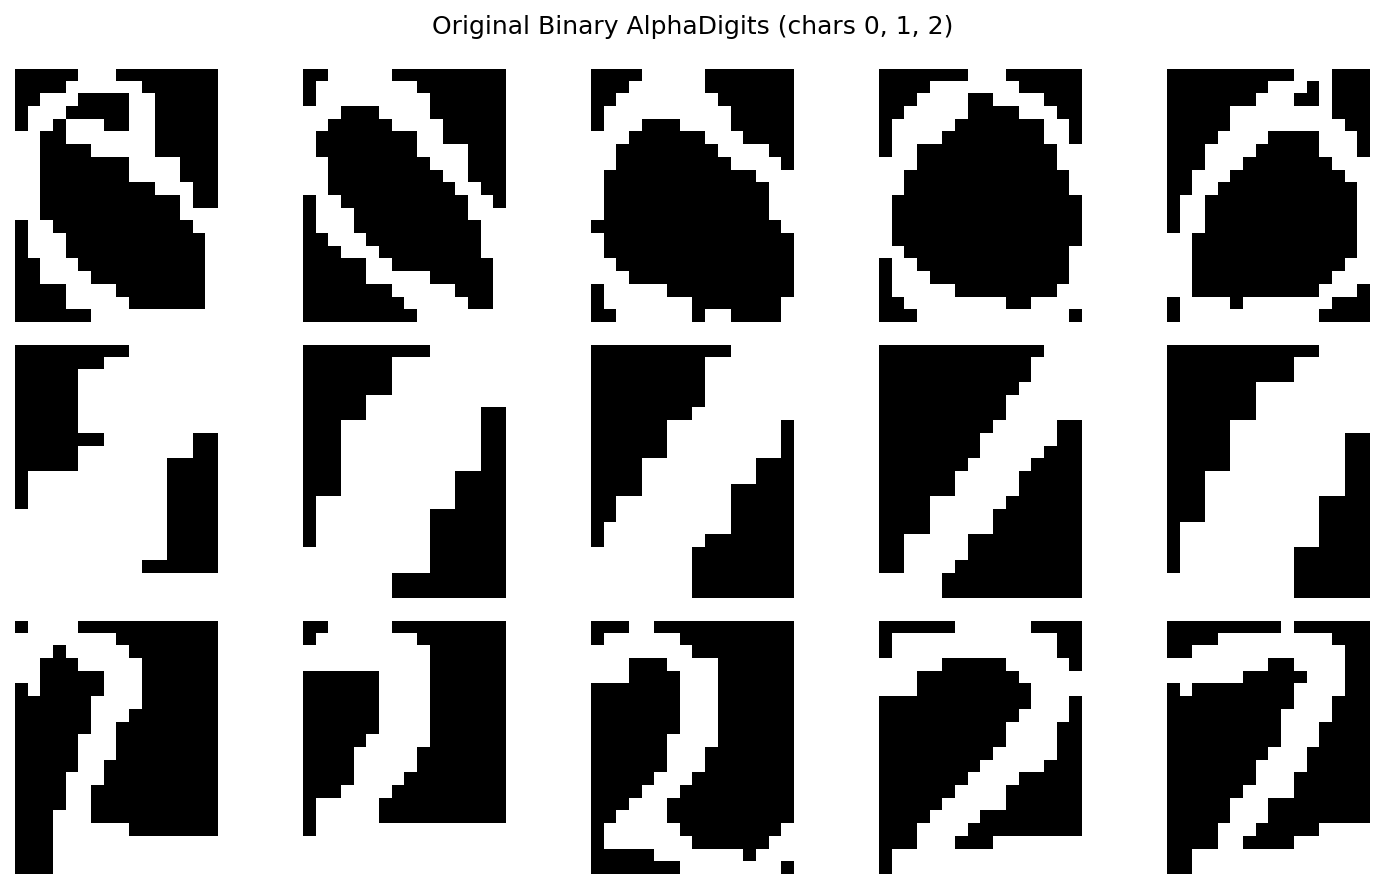
\includegraphics[width=0.8\linewidth]{alpha_originals.png}
    \caption{\'Echantillons originaux de Binary AlphaDigits (caract\`eres 0, 1, 2).}
    \label{fig:alpha_originals}
\end{figure}

\subsubsection{Effet du nombre d'unit\'es cach\'ees}

Nous entra\^inons des RBM avec $q \in \{50, 100, 200, 300\}$ unit\'es cach\'ees (100 \'epoques, $\eta = 0.1$, taille de batch 32) en utilisant l'algorithme de Divergence Contrastive (CD-1)~\cite{hinton2002} et g\'en\'erons des images via 500 pas de Gibbs.

\begin{figure}[H]
    \centering
    \begin{subfigure}{0.48\linewidth}
        \centering
        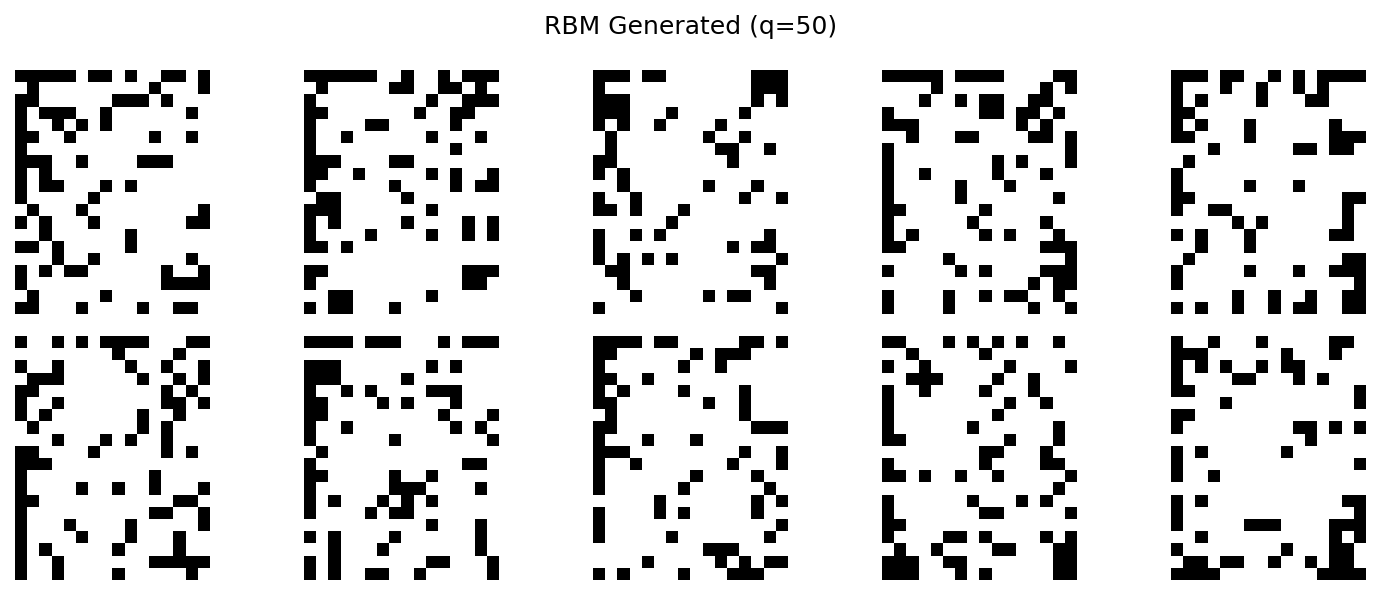
\includegraphics[width=\linewidth]{rbm_alpha_q50.png}
        \caption{$q = 50$}
    \end{subfigure}
    \hfill
    \begin{subfigure}{0.48\linewidth}
        \centering
        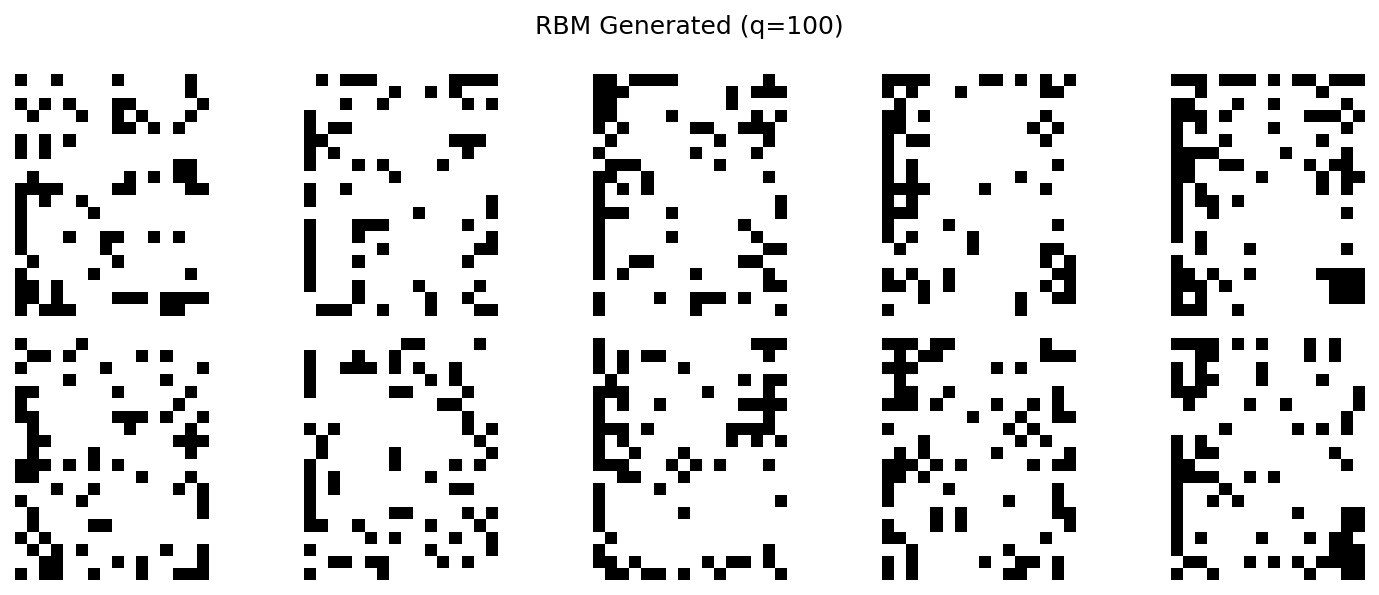
\includegraphics[width=\linewidth]{rbm_alpha_q100.png}
        \caption{$q = 100$}
    \end{subfigure}

    \vspace{0.3cm}

    \begin{subfigure}{0.48\linewidth}
        \centering
        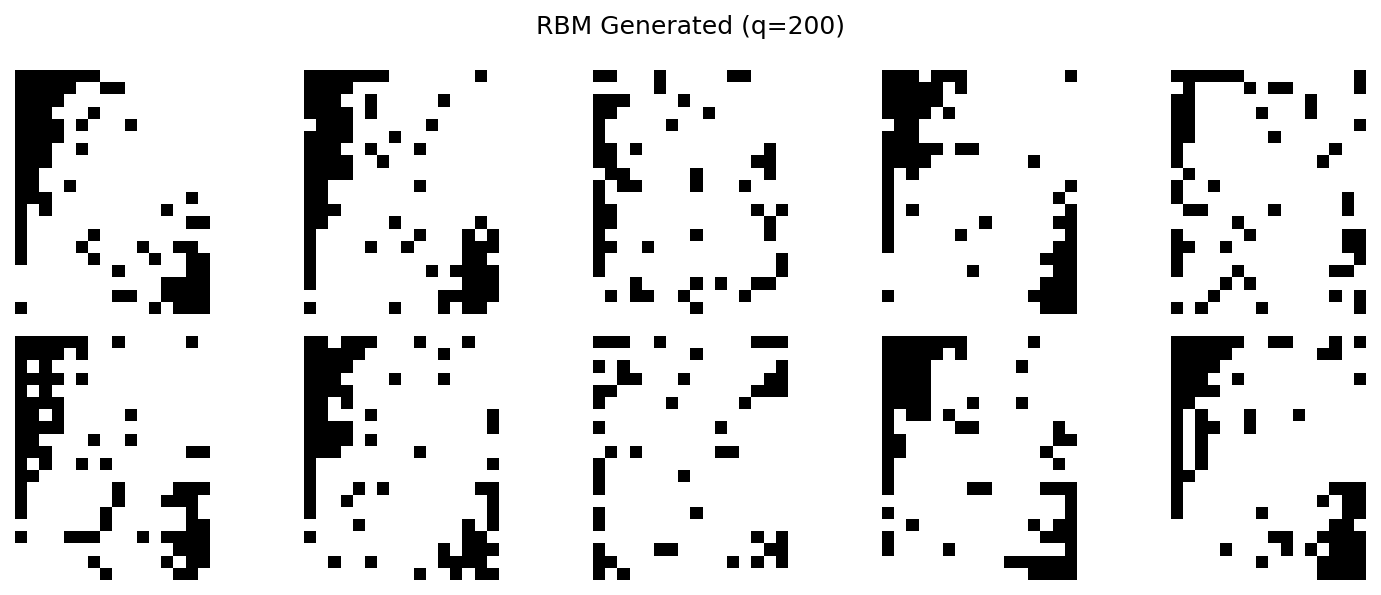
\includegraphics[width=\linewidth]{rbm_alpha_q200.png}
        \caption{$q = 200$}
    \end{subfigure}
    \hfill
    \begin{subfigure}{0.48\linewidth}
        \centering
        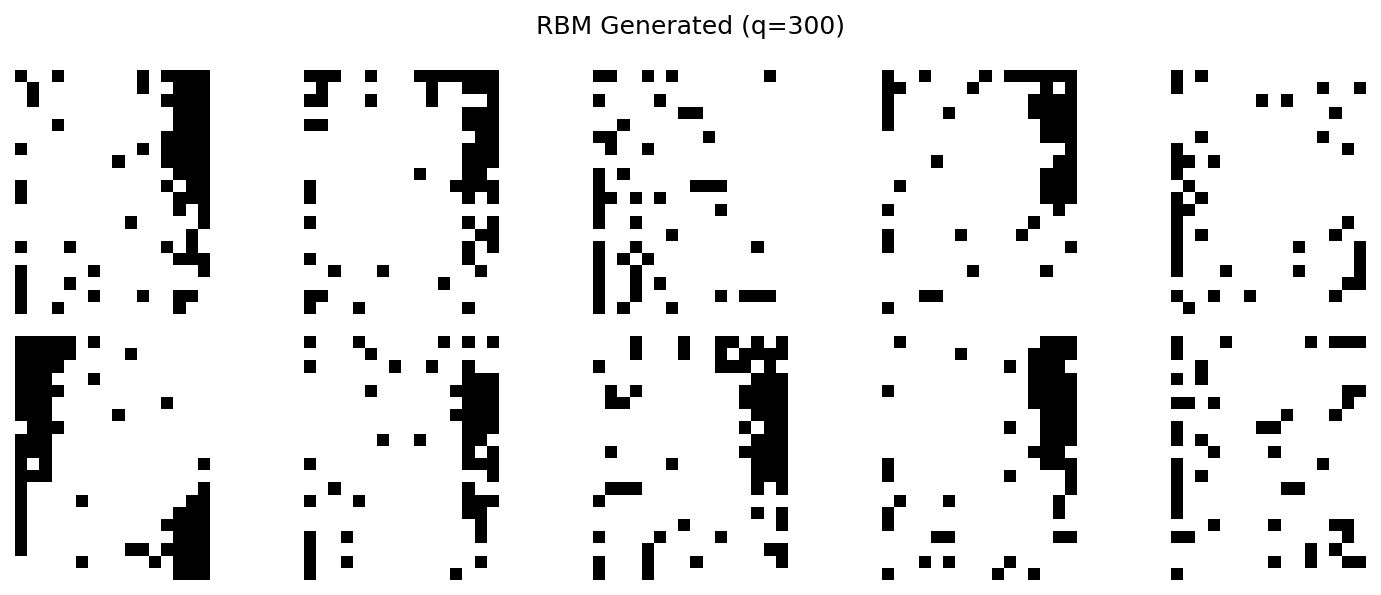
\includegraphics[width=\linewidth]{rbm_alpha_q300.png}
        \caption{$q = 300$}
    \end{subfigure}
    \caption{Images g\'en\'er\'ees par le RBM en fonction du nombre d'unit\'es cach\'ees $q$.}
    \label{fig:rbm_q}
\end{figure}

Avec $q = 50$, les images g\'en\'er\'ees sont tr\`es bruit\'ees avec quasiment aucune structure discernable, indiquant une capacit\'e insuffisante pour capturer la distribution des donn\'ees. \`A $q = 100$, une certaine structure locale commence \`a \'emerger : des r\'egions noires contigu\"es et des contours deviennent visibles, bien que les images restent bruit\'ees. Avec $q = 200$ et $q = 300$, les images g\'en\'er\'ees montrent des structures de blocs plus nettes rappelant les caract\`eres d'entra\^inement, avec des traits verticaux et diagonaux reconnaissables. L'am\'elioration de 200 \`a 300 est marginale, sugg\'erant que $q = 200$ offre un bon compromis entre capacit\'e et la taille limit\'ee de l'ensemble d'entra\^inement (117 \'echantillons). N\'eanmoins, la nature stochastique binaire du processus d'\'echantillonnage de Gibbs produit intrins\`equement des sorties bruit\'ees.

\subsubsection{Effet de la diversit\'e des caract\`eres}

Nous fixons $q = 200$ et varions le nombre de caract\`eres utilis\'es pour l'entra\^inement~: 3, 10 et 36 (tous les caract\`eres alphanum\'eriques).

\begin{figure}[H]
    \centering
    \begin{subfigure}{0.32\linewidth}
        \centering
        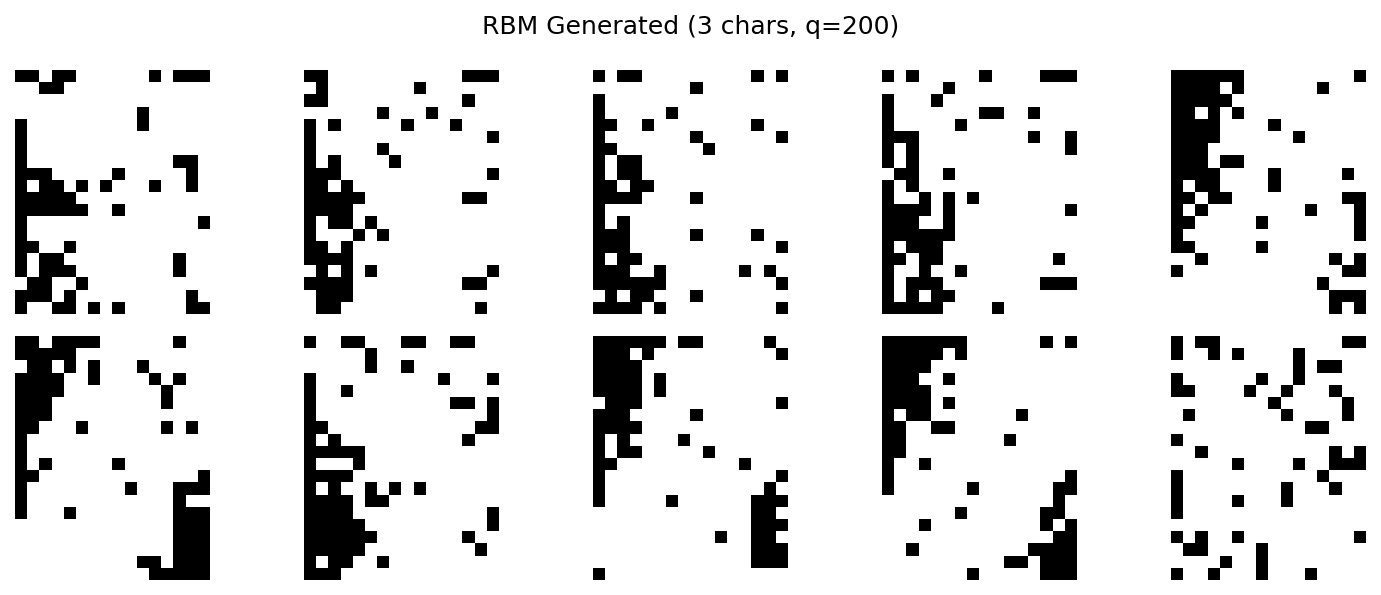
\includegraphics[width=\linewidth]{rbm_alpha_nchars3.png}
        \caption{3 caract\`eres}
    \end{subfigure}
    \hfill
    \begin{subfigure}{0.32\linewidth}
        \centering
        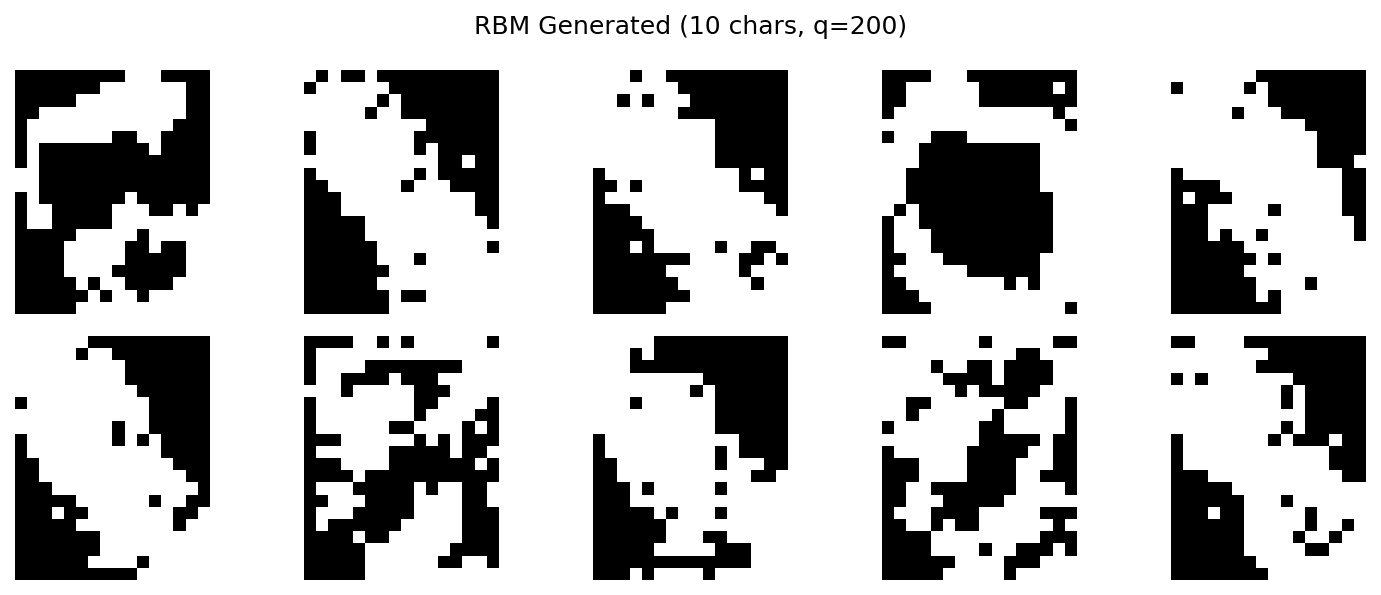
\includegraphics[width=\linewidth]{rbm_alpha_nchars10.png}
        \caption{10 caract\`eres}
    \end{subfigure}
    \hfill
    \begin{subfigure}{0.32\linewidth}
        \centering
        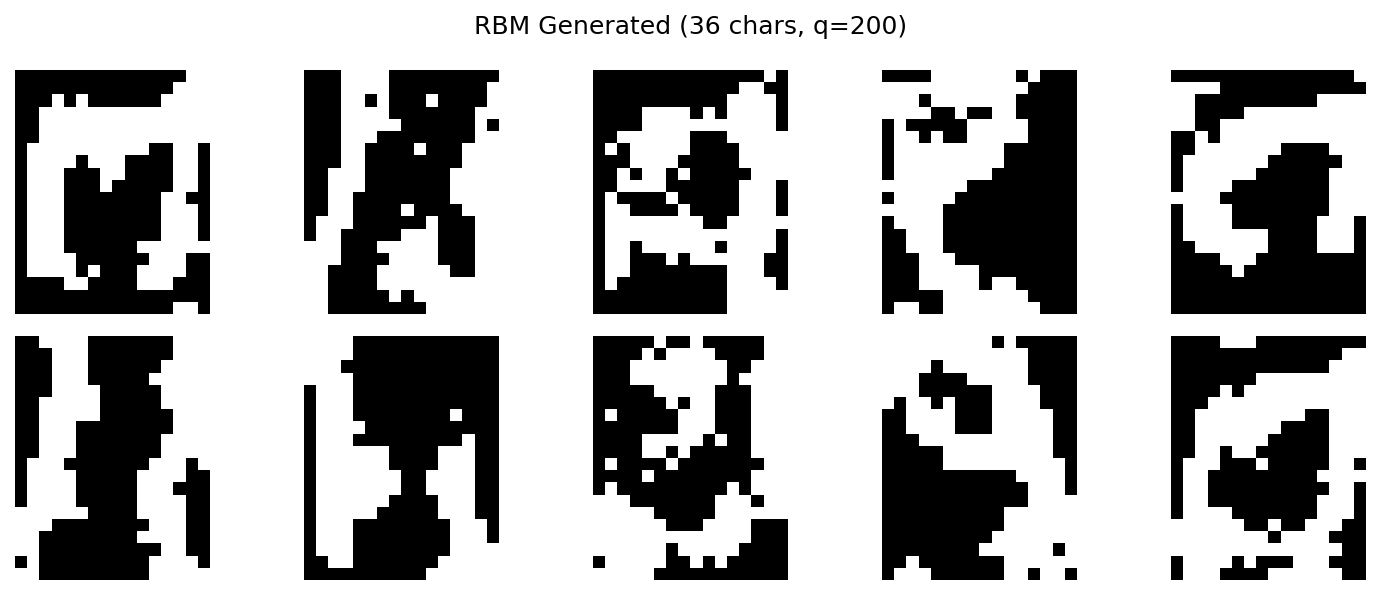
\includegraphics[width=\linewidth]{rbm_alpha_nchars36.png}
        \caption{36 caract\`eres}
    \end{subfigure}
    \caption{Images g\'en\'er\'ees par le RBM en fonction du nombre de caract\`eres d'entra\^inement ($q = 200$).}
    \label{fig:rbm_nchars}
\end{figure}

Avec 3 caract\`eres, les images g\'en\'er\'ees capturent certaines caract\'eristiques structurelles des chiffres mais restent bruit\'ees en raison du tr\`es petit ensemble d'entra\^inement (117 \'echantillons). De mani\`ere int\'eressante, avec 36 caract\`eres (1\,404 \'echantillons), les images g\'en\'er\'ees apparaissent plus structur\'ees, avec des formes de caract\`eres plus nettes. Cela s'explique par le fait que plus de donn\'ees d'entra\^inement permettent au RBM d'apprendre des caract\'eristiques plus robustes, m\^eme si la distribution est plus diverse. Le volume accru de donn\'ees compense la complexit\'e ajout\'ee, soulignant que la qualit\'e du RBM d\'epend fortement d'un nombre suffisant d'\'echantillons d'entra\^inement.

% ------------------------------------------------------------
\subsection{Exp\'eriences DBN}
\label{sec:dbn_alpha}
% ------------------------------------------------------------

\subsubsection{Effet de la profondeur du r\'eseau}

Nous entra\^inons des DBN~\cite{hinton2006} avec 1, 2 et 3 couches cach\'ees sur les caract\`eres 0, 1, 2, en utilisant l'entra\^inement glouton couche par couche~\cite{bengio2007}.

\begin{figure}[H]
    \centering
    \begin{subfigure}{0.32\linewidth}
        \centering
        
\includegraphics[width=\linewidth]{dbn_alpha_1layer.png}
        \caption{1 couche~: $320 \to 200$}
    \end{subfigure}
    \hfill
    \begin{subfigure}{0.32\linewidth}
        \centering
        
\includegraphics[width=\linewidth]{dbn_alpha_2layers.png}
        \caption{2 couches~: $320 \to 200 \to 100$}
    \end{subfigure}
    \hfill
    \begin{subfigure}{0.32\linewidth}
        \centering
        
\includegraphics[width=\linewidth]{dbn_alpha_3layers.png}
        \caption{3 couches~: $320 \to 200 \to 100 \to 50$}
    \end{subfigure}
    \caption{Images g\'en\'er\'ees par le DBN avec une profondeur variable.}
    \label{fig:dbn_layers}
\end{figure}

Le DBN \`a une seule couche (\'equivalent \`a un RBM) produit des images binaires bruit\'ees, similaires \`a celles du RBM isol\'e. Le \textbf{DBN \`a 2 couches} produit les meilleurs r\'esultats~: la propagation descendante \`a travers deux couches de probabilit\'es apprises g\'en\`ere des images en niveaux de gris lisses avec des formes de chiffres clairement reconnaissables (les 0 et les 2 sont distinctement visibles). Cela d\'emontre l'avantage de l'apprentissage hi\'erarchique de caract\'eristiques --- la premi\`ere couche capture la structure de bas niveau tandis que la seconde capture des abstractions de plus haut niveau. Le DBN \`a 3 couches, en revanche, produit des images en niveaux de gris floues et moins distinctes. Le RBM sup\'erieur op\`ere sur seulement 50 unit\'es cach\'ees, ce qui limite l'expressivit\'e de l'\'echantillonnage de Gibbs et conduit \`a des repr\'esentations de la couche sup\'erieure moins informatives propag\'ees vers le bas.

\subsubsection{Effet de la diversit\'e des caract\`eres sur le DBN}

Nous fixons l'architecture \`a $320 \to 200 \to 100$ et varions le nombre de caract\`eres.

\begin{figure}[H]
    \centering
    \begin{subfigure}{0.32\linewidth}
        \centering
        
\includegraphics[width=\linewidth]{dbn_alpha_nchars5.png}
        \caption{5 caract\`eres}
    \end{subfigure}
    \hfill
    \begin{subfigure}{0.32\linewidth}
        \centering
        
\includegraphics[width=\linewidth]{dbn_alpha_nchars10.png}
        \caption{10 caract\`eres}
    \end{subfigure}
    \hfill
    \begin{subfigure}{0.32\linewidth}
        \centering
        
\includegraphics[width=\linewidth]{dbn_alpha_nchars36.png}
        \caption{36 caract\`eres}
    \end{subfigure}
    \caption{Images g\'en\'er\'ees par le DBN en fonction du nombre de caract\`eres d'entra\^inement.}
    \label{fig:dbn_nchars}
\end{figure}

Le DBN \`a 2 couches produit des images en niveaux de gris lisses pour tous les niveaux de diversit\'e. Avec 5 caract\`eres, les images g\'en\'er\'ees sont les plus reconnaissables. Lorsque le nombre de caract\`eres augmente \`a 36, les images g\'en\'er\'ees deviennent plus uniformes et moins sp\'ecifiques \`a une classe, car le mod\`ele moyenne sur une distribution plus large. Compar\'e au RBM isol\'e, la structure hi\'erarchique du DBN et la propagation descendante bas\'ee sur les probabilit\'es produisent syst\'ematiquement des sorties plus lisses et plus reconnaissables, confirmant l'avantage des mod\`eles g\'en\'eratifs profonds m\^eme sur ce petit jeu de donn\'ees.

% ============================================================
\section{\'Etude sur MNIST}
\label{sec:dnn_mnist}
% ============================================================

Nous passons maintenant \`a l'\'etude principale~: comparer un DNN pr\'e-entra\^in\'e (pr\'e-entra\^inement non supervis\'e par RBM + r\'etropropagation) \`a un DNN initialis\'e al\'eatoirement (r\'etropropagation uniquement) sur MNIST.

\subsection{Protocole exp\'erimental}

Les images MNIST sont binaras\'ees au seuil 127. Pour chaque exp\'erience, deux DNN identiques sont cr\'e\'es. L'un est pr\'e-entra\^in\'e par entra\^inement glouton couche par couche de RBM (100 \'epoques par couche), puis ajust\'e par r\'etropropagation (200 \'epoques). L'autre est entra\^in\'e \`a partir d'une initialisation al\'eatoire avec r\'etropropagation uniquement (200 \'epoques). Les deux utilisent un taux d'apprentissage $\eta = 0.1$ et une taille de batch de 128. Le taux d'erreur de classification sur l'ensemble de test est rapport\'e.

Trois exp\'eriences sont r\'ealis\'ees conform\'ement au sujet~:

\subsection{Figure 1~: Taux d'erreur en fonction du nombre de couches cach\'ees}

Nous fixons le nombre de neurones par couche cach\'ee \`a 200 et varions le nombre de couches cach\'ees de 2 \`a 5. L'architecture est $[784, 200, \ldots, 200, 10]$.

\begin{figure}[H]
    \centering
    
\includegraphics[width=0.75\linewidth]{fig1_layers.png}
    \caption{Taux d'erreur de classification sur l'ensemble de test en fonction du nombre de couches cach\'ees (200 neurones chacune). Bleu~: pr\'e-entra\^in\'e + r\'etropropagation. Rouge~: initialisation al\'eatoire + r\'etropropagation.}
    \label{fig:fig1}
\end{figure}

\begin{table}[H]
\centering
\caption{Taux d'erreur en fonction du nombre de couches cach\'ees (200 neurones chacune).}
\label{tab:fig1}
\begin{tabular}{ccccc}
\toprule
Couches cach\'ees & \multicolumn{2}{c}{Erreur test (\%)} & \multicolumn{2}{c}{Erreur entra\^in. (\%)} \\
\cmidrule(lr){2-3} \cmidrule(lr){4-5}
 & Pr\'e-entra\^in\'e & Al\'eatoire & Pr\'e-entra\^in\'e & Al\'eatoire \\
\midrule
2 & 3.31 & \textbf{2.60} & 0.22 & 0.01 \\
3 & \textbf{2.84} & 3.39 & 0.12 & 0.07 \\
4 & \textbf{2.65} & 7.69 & 0.07 & 5.37 \\
5 & \textbf{2.63} & 88.65 & 0.06 & 88.76 \\
\bottomrule
\end{tabular}
\end{table}

\textbf{Analyse.} Avec 2 couches cach\'ees, le r\'eseau al\'eatoire surpasse l\'eg\`erement le r\'eseau pr\'e-entra\^in\'e (2.60\,\% contre 3.31\,\%). Cependant, lorsque la profondeur augmente, le r\'eseau initialis\'e al\'eatoirement se d\'egrade de mani\`ere dramatique~: \`a 4 couches il atteint 7.69\,\% d'erreur, et \`a 5 couches la perte reste bloqu\'ee \`a $\approx 2.30$ ($= \ln 10$, c'est-\`a-dire une pr\'ediction al\'eatoire) pendant les 200 \'epoques d'entra\^inement, donnant $\approx 90\,\%$ d'erreur.

Ceci est une d\'emonstration classique du \textbf{probl\`eme du gradient \'evanescent}~\cite{erhan2010}~: dans les r\'eseaux profonds initialis\'es al\'eatoirement, les gradients deviennent extr\^emement petits dans les couches ant\'erieures, emp\^echant tout apprentissage. Le plateau de la perte \`a $\ln(10)$ confirme que le r\'eseau produit des probabilit\'es softmax uniformes. En revanche, le r\'eseau pr\'e-entra\^in\'e maintient des performances stables et m\^eme l\'eg\`erement am\'elior\'ees lorsque la profondeur augmente (2.65\,\% \`a 4 couches), car le pr\'e-entra\^inement par RBM place les poids dans une r\'egion favorable de l'espace des param\`etres o\`u les gradients circulent efficacement.

Le point cl\'e est que le \textbf{pr\'e-entra\^inement est essentiel pour les architectures profondes} (plus de 2--3 couches cach\'ees). Pour les r\'eseaux peu profonds (2 couches), l'initialisation al\'eatoire est comp\'etitive. Pour notre meilleur mod\`ele, nous s\'electionnons \textbf{2 couches cach\'ees} car les r\'eseaux plus profonds n'am\'eliorent pas l'erreur de test malgr\'e le pr\'e-entra\^inement.

\subsection{Figure 2~: Taux d'erreur en fonction du nombre de neurones par couche}

Nous fixons l'architecture \`a 2 couches cach\'ees et varions le nombre de neurones par couche~: 100, 300, 500 et 700.

\begin{figure}[H]
    \centering
    
\includegraphics[width=0.75\linewidth]{fig2_neurons.png}
    \caption{Taux d'erreur de classification en fonction du nombre de neurones par couche cach\'ee (2 couches cach\'ees). Bleu~: pr\'e-entra\^in\'e. Rouge~: init. al\'eatoire.}
    \label{fig:fig2}
\end{figure}

\begin{table}[H]
\centering
\caption{Taux d'erreur en fonction du nombre de neurones par couche cach\'ee (2 couches cach\'ees).}
\label{tab:fig2}
\begin{tabular}{ccccc}
\toprule
Neurones/couche & \multicolumn{2}{c}{Erreur test (\%)} & \multicolumn{2}{c}{Erreur entra\^in. (\%)} \\
\cmidrule(lr){2-3} \cmidrule(lr){4-5}
 & Pr\'e-entra\^in\'e & Al\'eatoire & Pr\'e-entra\^in\'e & Al\'eatoire \\
\midrule
100 & 4.06 & \textbf{2.86} & 1.16 & 0.01 \\
300 & 3.45 & \textbf{2.69} & 0.06 & 0.02 \\
500 & 3.10 & \textbf{2.67} & 0.01 & 0.04 \\
700 & \textbf{2.48} & 2.67 & 0.00 & 0.07 \\
\bottomrule
\end{tabular}
\end{table}

\textbf{Analyse.} Un motif int\'eressant \'emerge~: pour les petites et moyennes largeurs (100--500 neurones), le r\'eseau initialis\'e al\'eatoirement surpasse en fait le r\'eseau pr\'e-entra\^in\'e sur l'ensemble de test. Cependant, le r\'eseau pr\'e-entra\^in\'e s'am\'eliore de mani\`ere constante avec plus de neurones, et \`a 700 neurones il d\'epasse finalement le r\'eseau al\'eatoire (2.48\,\% contre 2.67\,\%).

Cela peut s'expliquer en examinant les erreurs d'entra\^inement~: le r\'eseau pr\'e-entra\^in\'e avec 100 neurones a une erreur d'entra\^inement relativement \'elev\'ee (1.16\,\%), sugg\'erant que le pr\'e-entra\^inement peut imposer une initialisation trop rigide pour les petits r\'eseaux, limitant leur flexibilit\'e lors de la r\'etropropagation. Lorsque la largeur augmente, le r\'eseau pr\'e-entra\^in\'e peut mieux exploiter les caract\'eristiques plus riches apprises durant la phase non supervis\'ee, atteignant finalement 0\,\% d'erreur d'entra\^inement et la meilleure erreur de test \`a 700 neurones. Le r\'eseau al\'eatoire plafonne \`a $\approx 2.67\,\%$ d'erreur de test quelle que soit la largeur au-del\`a de 300 neurones. Pour notre meilleur mod\`ele, \textbf{700 neurones par couche} est optimal.

\subsection{Figure 3~: Taux d'erreur en fonction du nombre d'\'echantillons d'entra\^inement}

Nous fixons l'architecture \`a $[784, 200, 200, 10]$ et varions le nombre d'\'echantillons d'entra\^inement~: 1\,000, 3\,000, 7\,000, 10\,000, 30\,000 et 60\,000.

\begin{figure}[H]
    \centering
    
\includegraphics[width=0.75\linewidth]{fig3_samples.png}
    \caption{Taux d'erreur de classification en fonction du nombre d'\'echantillons d'entra\^inement (\'echelle logarithmique). Architecture~: $[784, 200, 200, 10]$.}
    \label{fig:fig3}
\end{figure}

\begin{table}[H]
\centering
\caption{Taux d'erreur en fonction du nombre d'\'echantillons d'entra\^inement. Architecture~: $[784, 200, 200, 10]$.}
\label{tab:fig3}
\begin{tabular}{ccccc}
\toprule
\'Echantillons & \multicolumn{2}{c}{Erreur test (\%)} & \multicolumn{2}{c}{Erreur entra\^in. (\%)} \\
\cmidrule(lr){2-3} \cmidrule(lr){4-5}
 & Pr\'e-entra\^in\'e & Al\'eatoire & Pr\'e-entra\^in\'e & Al\'eatoire \\
\midrule
1\,000  & \textbf{10.10} & 90.26 & 2.50  & 88.50 \\
3\,000  & \textbf{7.01}  & 19.25 & 1.43  & 15.17 \\
7\,000  & \textbf{6.20}  & 9.75  & 0.93  & 4.13  \\
10\,000 & \textbf{5.69}  & 7.86  & 0.69  & 2.81  \\
60\,000 & 3.31           & \textbf{2.60} & 0.22  & 0.01  \\
\bottomrule
\end{tabular}
\end{table}

\textbf{Analyse.} Le pr\'e-entra\^inement apporte son plus grand avantage dans le \textbf{r\'egime de donn\'ees limit\'ees}. Avec seulement 1\,000 \'echantillons d'entra\^inement, le r\'eseau initialis\'e al\'eatoirement est compl\`etement bloqu\'e \`a $\approx 90\,\%$ d'erreur (la perte reste \`a $\ln(10) \approx 2.30$ tout au long de l'entra\^inement, c'est-\`a-dire une pr\'ediction al\'eatoire), tandis que le r\'eseau pr\'e-entra\^in\'e atteint 10.10\,\%. M\^eme avec 3\,000 \'echantillons, l'\'ecart est consid\'erable~: 7.01\,\% contre 19.25\,\%.

\`A mesure que le jeu de donn\'ees cro\^it, l'\'ecart se r\'eduit. Avec 10\,000 \'echantillons, le r\'eseau al\'eatoire commence \`a apprendre efficacement (7.86\,\%), et \`a 60\,000 \'echantillons il surpasse en fait le r\'eseau pr\'e-entra\^in\'e (2.60\,\% contre 3.31\,\%).

Cela est coh\'erent avec la th\'eorie~\cite{erhan2010}~: le pr\'e-entra\^inement non supervis\'e agit comme un r\'egulariseur en apprenant la structure de la distribution des entr\'ees. Lorsque les donn\'ees \'etiquet\'ees sont rares, cette connaissance a priori est critique; sans elle, le r\'eseau initialis\'e al\'eatoirement ne peut m\^eme pas \'echapper au plateau de pr\'ediction al\'eatoire. Avec des donn\'ees \'etiquet\'ees abondantes, l'entra\^inement supervis\'e seul peut d\'ecouvrir des caract\'eristiques comparables, rendant le pr\'e-entra\^inement superflu. Pour notre meilleur mod\`ele, nous utilisons \textbf{les 60\,000 \'echantillons d'entra\^inement}.

\subsection{Configuration du meilleur mod\`ele}
\label{sec:best_model}

Sur la base des trois exp\'eriences ci-dessus, la configuration optimale est~:

\begin{itemize}
    \item \textbf{Architecture}~: $[784, 700, 700, 10]$ : 2 couches cach\'ees (Fig.~1) avec 700 neurones chacune (Fig.~2)
    \item \textbf{Pr\'e-entra\^inement}~: Oui, syst\'ematiquement meilleur ou \'egal \`a l'initialisation al\'eatoire
    \item \textbf{Donn\'ees d'entra\^inement}~: Les 60\,000 \'echantillons (Fig.~3)
    \item \textbf{Pr\'e-entra\^inement RBM}~: 100 \'epoques par couche, $\eta = 0.1$
    \item \textbf{R\'etropropagation}~: 200 \'epoques, $\eta = 0.1$, taille de batch 128
\end{itemize}

\begin{figure}[H]
    \centering
    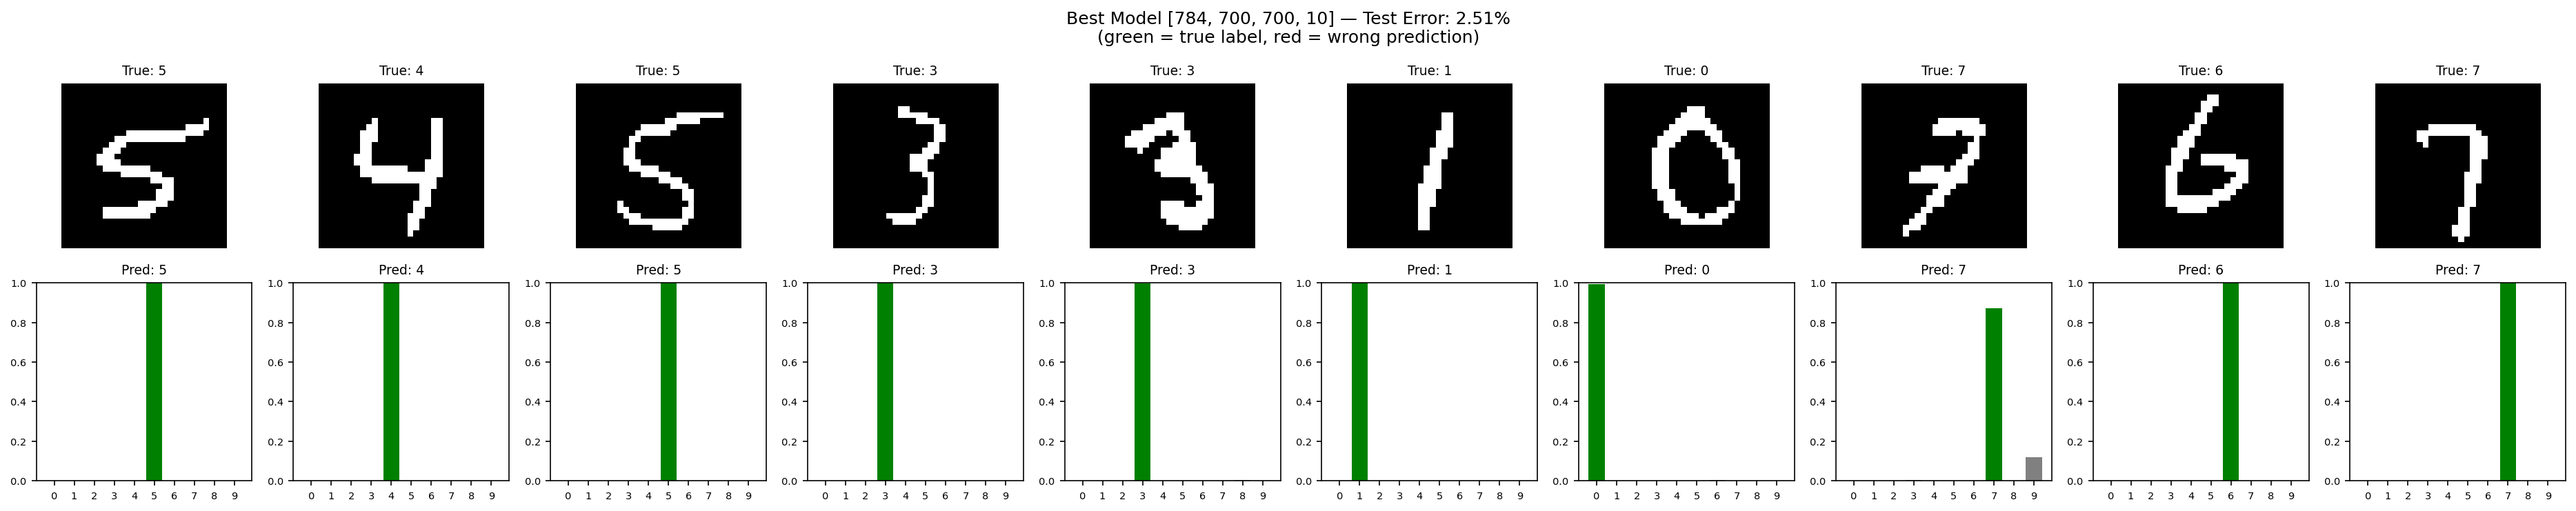
\includegraphics[width=\linewidth]{softmax_best_model.png}
    \caption{Pr\'edictions du meilleur mod\`ele sur des \'echantillons de test al\'eatoires. Ligne du haut~: image d'entr\'ee avec le vrai label. Ligne du bas~: probabilit\'es softmax en sortie (vert = vrai label, rouge = pr\'ediction incorrecte).}
    \label{fig:softmax}
\end{figure}

Le meilleur mod\`ele atteint un taux d'erreur de test de \textbf{2.51\,\%}. Les probabilit\'es softmax en sortie (Figure~\ref{fig:softmax}) montrent des pr\'edictions confiantes et bien calibr\'ees, avec la masse de probabilit\'e concentr\'ee presque enti\`erement sur la classe correcte. Les 10 \'echantillons de test s\'electionn\'es al\'eatoirement dans la figure sont tous correctement class\'es avec une quasi-certitude.

% ============================================================
\section{Bonus~: Comparaison de mod\`eles g\'en\'eratifs}
\label{sec:bonus}
% ============================================================

En bonus, nous comparons cinq mod\`eles g\'en\'eratifs entra\^in\'es sur MNIST avec approximativement le m\^eme nombre de param\`etres ($\sim$160k chacun)~:

\begin{enumerate}
    \item \textbf{RBM} ($784 \to 200$, $\sim$158k param.)~: 100 \'epoques de CD-1, g\'en\'eration via 1\,000 pas de Gibbs.
    \item \textbf{DBN} ($784 \to 200 \to 100$, $\sim$178k param.)~: Entra\^inement glouton couche par couche, g\'en\'eration via Gibbs au sommet + propagation descendante.
    \item \textbf{VAE}~\cite{kingma2014} ($784 \to 200 \to 100 \to 20 \to 100 \to 200 \to 784$, $\sim$161k param.)~: Auto-encodeur variationnel avec astuce de reparam\'etrisation, entra\^in\'e pendant 200 \'epoques avec Adam.
    \item \textbf{GAN}~\cite{goodfellow2014} (G\'en\'erateur~: $64 \to 256 \to 512 \to 784$ avec BatchNorm~; Discriminateur~: $784 \to 512 \to 256 \to 1$ avec Dropout, $\sim$210k param. au total)~: Entra\^in\'e pendant 200 \'epoques avec label smoothing.
    \item \textbf{DDPM}~\cite{ho2020} (Mod\`ele de diffusion probabiliste par d\'ebruitage, $\sim$169k param.)~: D\'ebruiteur MLP simple avec embeddings temporels sinuso\"idaux, connexions r\'esiduelles, activations GELU, $T = 500$ \'etapes de diffusion, 200 \'epoques.
\end{enumerate}

Les VAE, GAN et DDPM sont impl\'ement\'es en PyTorch et entra\^in\'es sur Google Colab avec acc\'el\'eration GPU. Le RBM et le DBN utilisent notre impl\'ementation NumPy. Le notebook de comparaison est autonome et disponible \`a \texttt{notebooks/bonus\_comparison.ipynb}.

\begin{figure}[H]
    \centering
    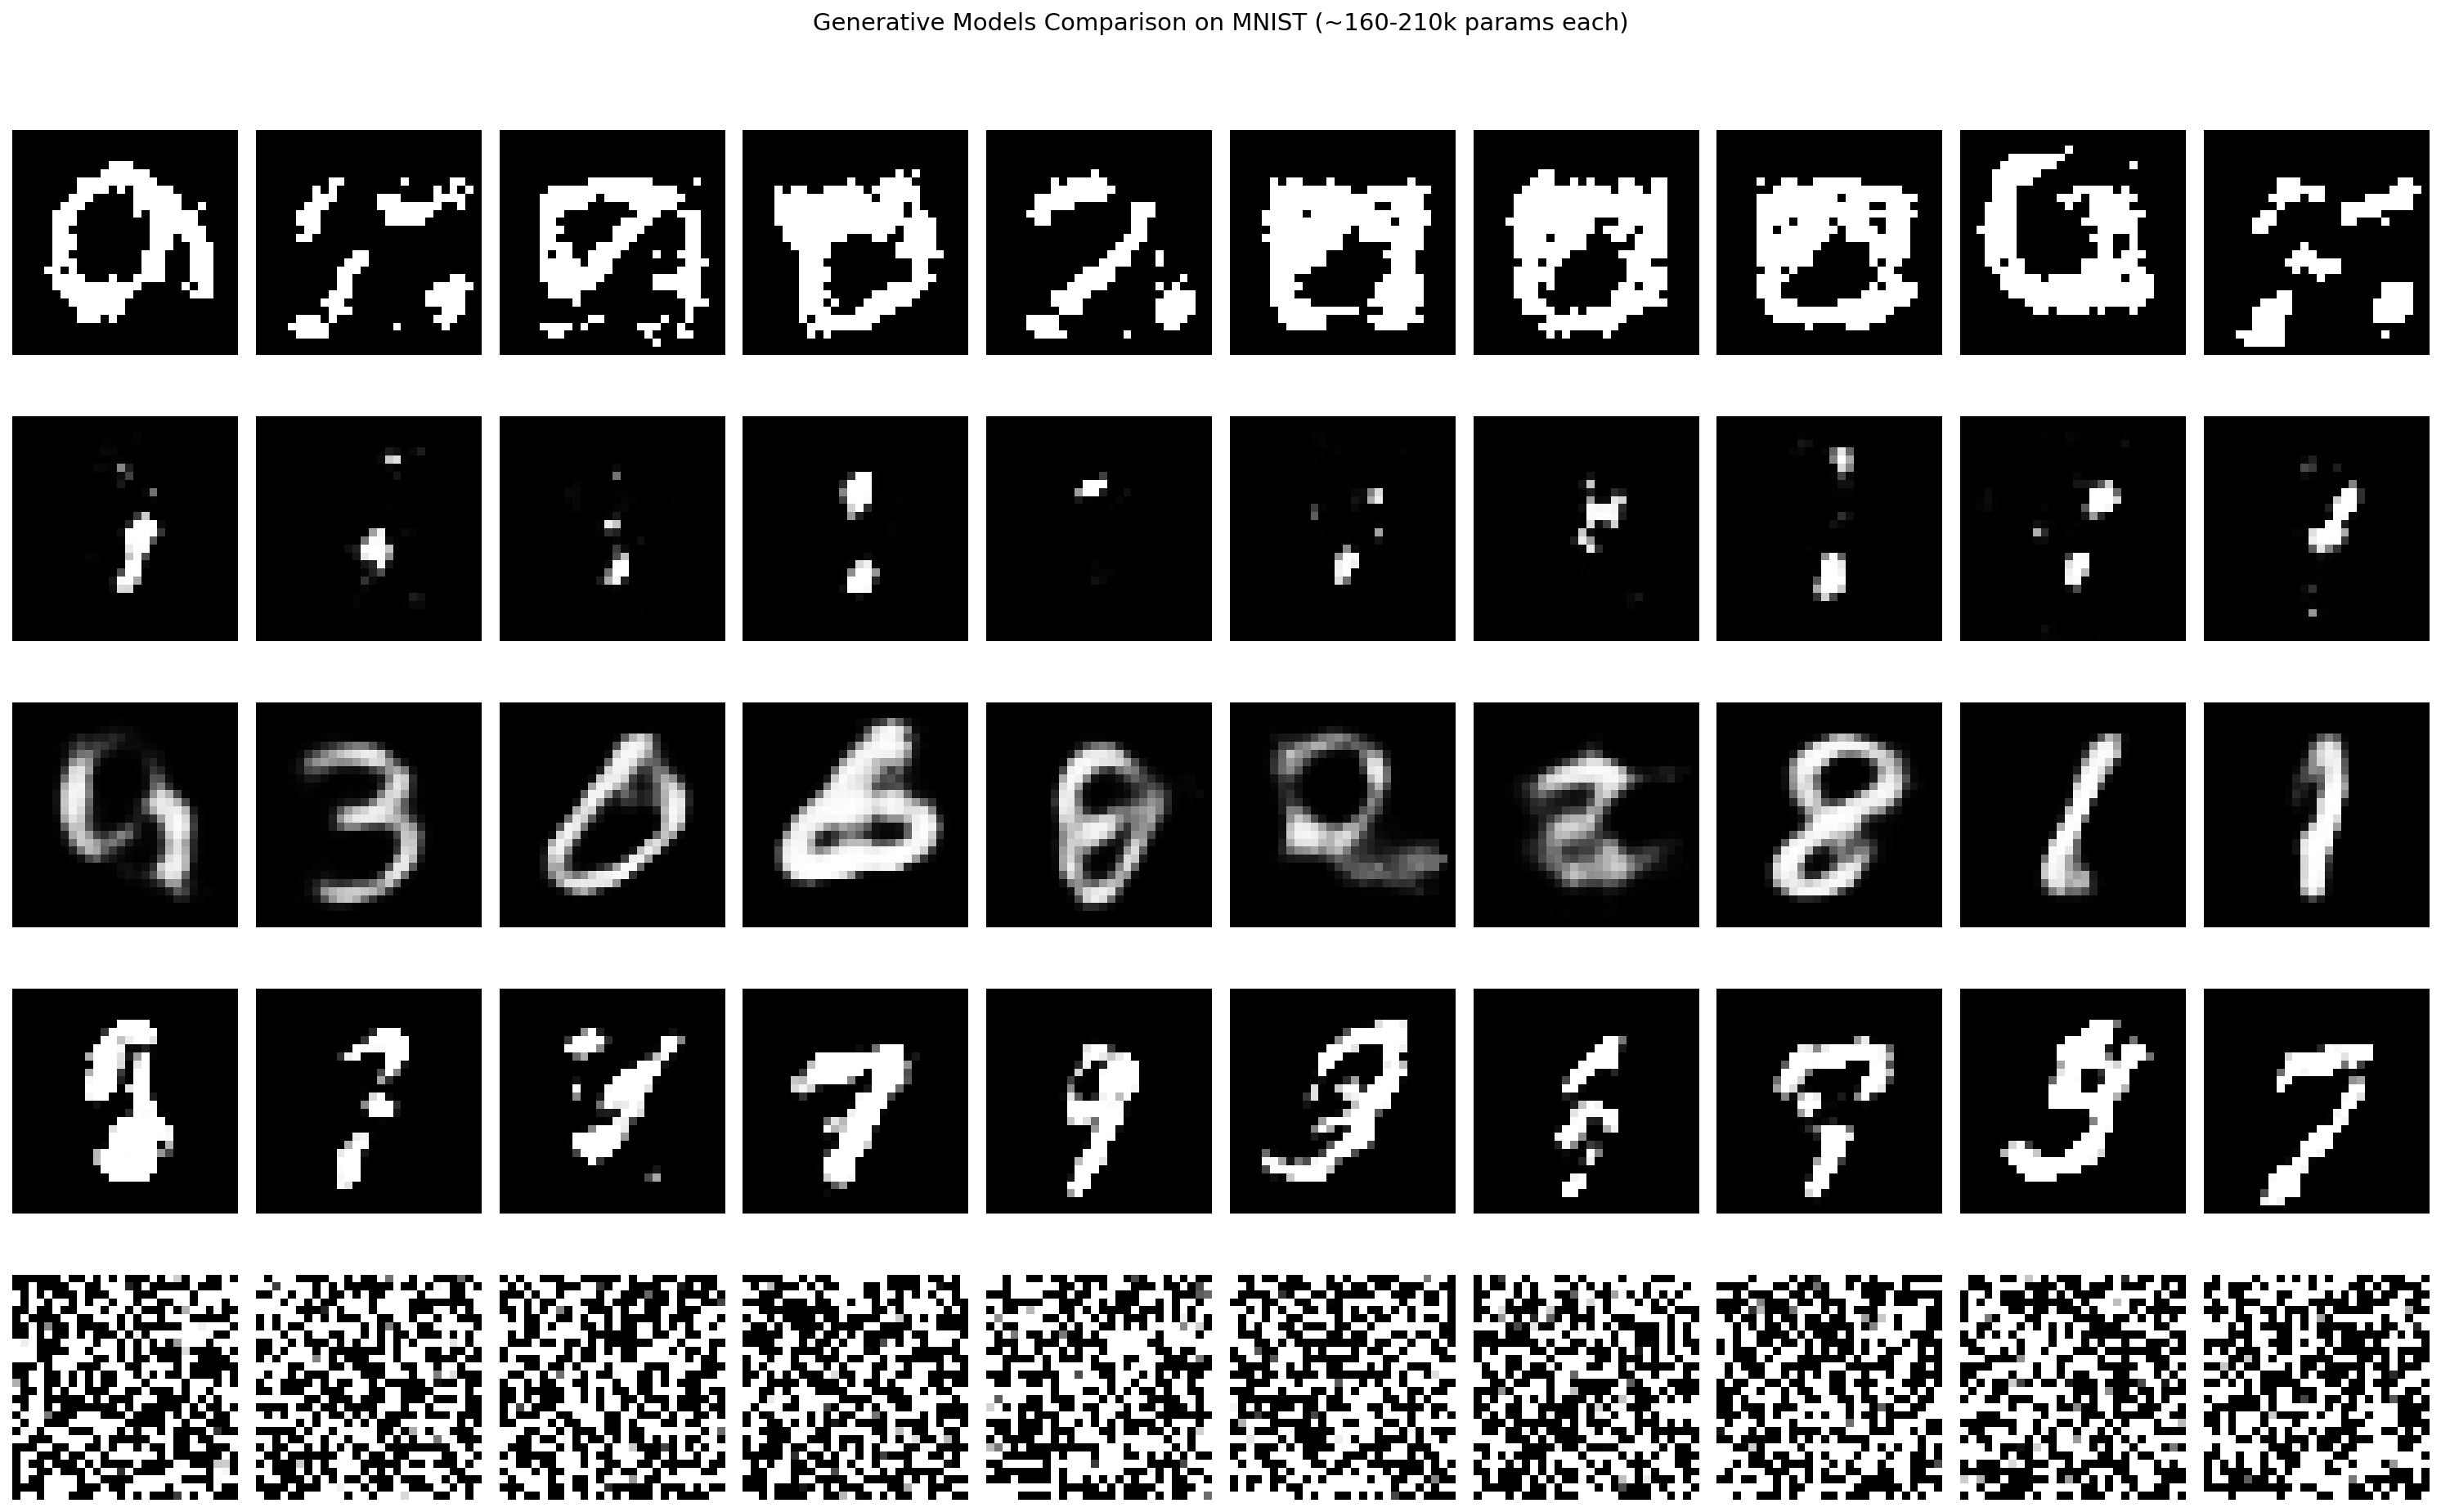
\includegraphics[width=\linewidth]{bonus_comparison.png}
    \caption{\'Echantillons MNIST g\'en\'er\'es par cinq mod\`eles g\'en\'eratifs avec approximativement le m\^eme budget de param\`etres. G\'en\'er\'es via le notebook Colab \texttt{notebooks/bonus\_comparison.ipynb}.}
    \label{fig:bonus}
\end{figure}
\noindent\textit{Note~: Cette figure est g\'en\'er\'ee en ex\'ecutant le notebook Colab, qui t\'el\'echarge MNIST et entra\^ine les cinq mod\`eles avec acc\'el\'eration GPU.}

\textbf{Analyse.}
\begin{itemize}
    \item Le \textbf{RBM} et le \textbf{DBN} produisent des chiffres reconnaissables mais bruit\'es d'apparence binaire, coh\'erent avec leur nature stochastique binaire.
    \item Le \textbf{VAE}~\cite{kingma2014} g\'en\`ere des chiffres lisses et plausibles avec une bonne diversit\'e, b\'en\'eficiant de l'espace latent continu et de l'objectif de reconstruction + KL.
    \item Le \textbf{GAN}~\cite{goodfellow2014} produit les images les plus nettes globalement, car l'entra\^inement adversarial optimise directement le r\'ealisme. Cependant, l'effondrement de modes peut parfois r\'eduire la diversit\'e.
    \item Le \textbf{DDPM}~\cite{ho2020} produit des chiffres raisonnables mais moins nets. C'est une limitation connue de l'utilisation d'une architecture MLP simple pour le d\'ebruitage~: le DDPM standard repose sur des architectures U-Net avec des convolutions spatiales et des m\'ecanismes d'attention, qui ne peuvent pas \^etre r\'epliqu\'ees dans le budget de $\sim$160k param\`etres. Le MLP peine \`a d\'ebruiter efficacement des vecteurs de dimension 784 compar\'e aux architectures convolutives qui exploitent la structure spatiale.
\end{itemize}

Cette comparaison illustre le compromis entre les familles de mod\`eles~: les RBM/DBN sont simples et th\'eoriquement fond\'es mais limit\'es en qualit\'e de sortie~; les VAE offrent un bon \'equilibre entre qualit\'e et stabilit\'e d'entra\^inement~; les GAN excellent en nettet\'e mais sont plus difficiles \`a entra\^iner~; et les mod\`eles de diffusion n\'ecessitent des architectures sp\'ecialis\'ees pour atteindre leur plein potentiel.

% ============================================================
\section{Conclusion}
% ============================================================

Ce projet a d\'emontr\'e le pipeline complet allant de l'apprentissage non supervis\'e de caract\'eristiques avec les RBM \`a la classification supervis\'ee avec les DNN sur MNIST. Les principaux r\'esultats sont~:

\begin{enumerate}
    \item \textbf{Le pr\'e-entra\^inement att\'enue le probl\`eme du gradient \'evanescent}~\cite{erhan2010} dans les r\'eseaux profonds, permettant l'entra\^inement efficace d'architectures avec 4--5 couches cach\'ees qui \'echoueraient autrement avec une initialisation al\'eatoire.
    \item \textbf{Pour les r\'eseaux peu profonds (2 couches), l'avantage du pr\'e-entra\^inement est marginal} lorsque suffisamment de donn\'ees \'etiquet\'ees sont disponibles, mais devient significatif dans le r\'egime de donn\'ees limit\'ees.
    \item \textbf{Les r\'eseaux pr\'e-entra\^in\'es passent mieux \`a l'\'echelle en largeur}~: augmenter les unit\'es cach\'ees \`a 700 donne une am\'elioration constante pour les r\'eseaux pr\'e-entra\^in\'es, tandis que les r\'eseaux initialis\'es al\'eatoirement plafonnent plus t\^ot.
    \item La \textbf{configuration optimale} pour la classification MNIST est $[784, 700, 700, 10]$ avec pr\'e-entra\^inement, atteignant $2.51\,\%$ d'erreur de test.
    \item Parmi les mod\`eles g\'en\'eratifs avec des budgets de param\`etres comparables, \textbf{les GAN produisent les \'echantillons les plus nets}, \textbf{les VAE offrent le meilleur compromis qualit\'e-stabilit\'e}, et \textbf{les mod\`eles de diffusion n\'ecessitent des architectures convolutives} pour atteindre leur potentiel.
\end{enumerate}

Tout le code est impl\'ement\'e from scratch en NumPy (partie principale) et PyTorch (bonus uniquement), organis\'e dans un package modulaire \texttt{src/} avec des scripts d'exp\'eriences reproductibles dans \texttt{experiments/}.

% ============================================================
\begin{thebibliography}{9}
% ============================================================

\bibitem{hinton2002}
Hinton, G.~E. (2002).
\textit{Training Products of Experts by Minimizing Contrastive Divergence}.
Neural Computation, 14(8), 1771--1800.

\bibitem{hinton2006}
Hinton, G.~E., Osindero, S. et Teh, Y.~W. (2006).
\textit{A Fast Learning Algorithm for Deep Belief Nets}.
Neural Computation, 18(7), 1527--1554.

\bibitem{erhan2010}
Erhan, D., Bengio, Y., Courville, A., Manzagol, P.-A., Vincent, P. et Bengio, S. (2010).
\textit{Why Does Unsupervised Pre-training Help Deep Learning?}
Journal of Machine Learning Research, 11, 625--660.

\bibitem{lecun1998}
LeCun, Y., Bottou, L., Bengio, Y. et Haffner, P. (1998).
\textit{Gradient-Based Learning Applied to Document Recognition}.
Proceedings of the IEEE, 86(11), 2278--2324.

\bibitem{kingma2014}
Kingma, D.~P. et Welling, M. (2014).
\textit{Auto-Encoding Variational Bayes}.
International Conference on Learning Representations (ICLR).

\bibitem{goodfellow2014}
Goodfellow, I., Pouget-Abadie, J., Mirza, M., Xu, B., Warde-Farley, D., Ozair, S., Courville, A. et Bengio, Y. (2014).
\textit{Generative Adversarial Nets}.
Advances in Neural Information Processing Systems (NeurIPS), 27.

\bibitem{ho2020}
Ho, J., Jain, A. et Abbeel, P. (2020).
\textit{Denoising Diffusion Probabilistic Models}.
Advances in Neural Information Processing Systems (NeurIPS), 33.

\bibitem{bengio2007}
Bengio, Y., Lamblin, P., Popovici, D. et Larochelle, H. (2007).
\textit{Greedy Layer-Wise Training of Deep Networks}.
Advances in Neural Information Processing Systems (NeurIPS), 19.

\bibitem{smolensky1986}
Smolensky, P. (1986).
\textit{Information Processing in Dynamical Systems: Foundations of Harmony Theory}.
Dans D.~E. Rumelhart et J.~L. McClelland (dir.), Parallel Distributed Processing, vol.~1, chap.~6, p.~194--281. MIT Press.

\end{thebibliography}

\end{document}
